%==========================================================================
%Template File for Monthly Lectual Meeting
%2006/05/22 (kkobayashi@mikilab.doshisha.ac.jp)
%==========================================================================
\documentclass[a4paper,9pt,twocolumn]{jsarticle}
\usepackage{mlm2.0}
\usepackage{epsf}
\pagestyle{plain}
\usepackage{url}
\usepackage{subfigure}
\setcounter{page}{1}
\usepackage{geometry}
\geometry{left=25mm,right=25mm,top=20mm,bottom=30mm}
%\usepackage[dvips]{graphicx}

\begin{document}
\twocolumn[
%---------------------------------------------------------------------------        % ヘッダ    書式:\beginheader{回}{年}{月}
%---------------------------------------------------------------------------
\beginheader{170}{2016}{04}
%---------------------------------------------------------------------------
% 発表題目    書式:\title{日本語}{英語} 「\\」で改行できます
%---------------------------------------------------------------------------
\title%
{git}%
%{更なる大容量化を目指して 進化しつづける次世代光メディア}

%---------------------------------------------------------------------------
% 著者名      書式:\author{日本語著者名}{英語著者名}
%---------------------------------------------------------------------------
\author{山下 俊樹,外村 篤紀\\Toshiki YAMASHITA,Atsuki TONOMURA}

%---------------------------------------------------------------------------
\endheader
%\begin{abstract}
%---------------------------------------------------------------------------
%Recently, a DVD attracts attention along with the image and the digitization of the sound. The standards of these DVD are complicated. So, in this paper, the standards of the DVD are summarized and the DVD of the next generation is refered. 
%---------------------------------------------------------------------------
%\end{abstract}
]

%---------------------------------------------------------------------------
% 本文
%---------------------------------------------------------------------------

\section{はじめに}
近年,ソフトウエアは大規模化し,修正を行う対象の数が増加したため,その更新頻度は増加の一途を辿っている.そこで,コンピューター上で作成,および編集されるファイルの変更履歴を管理するバージョン管理システムの重要性が増している.バージョン管理システムには,管理下のファイルを任意の記録時点の状態に復元することができる,および一つのファイルを複数人で編集する場合,競合が発生しないように管理が行われるなどの利点があるため,注目を集めている.

バージョン管理システムには,サーバ上のみでファイルの管理を行う集中型バージョン管理システムと,サーバに加え,個人のPCでも管理を行う分散型バージョン管理システムがある.本報告では,分散型バージョン管理システムの一つであるgitの概要,内部処理,および利点について述べる.

\section{git}
\subsection{gitの構成}
gitの構成を以下の\fgref{git}に示す.

\begin{figure}[h]
\centering
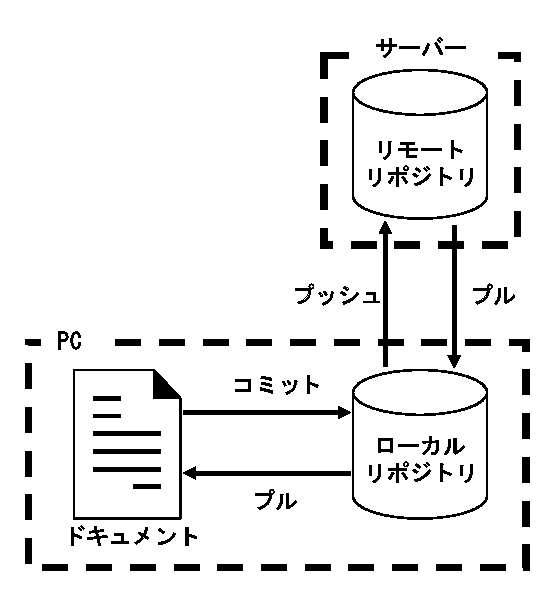
\includegraphics[height=50mm]{img/git.eps}
\caption{gitの構成}
\label{git}
\end{figure}

gitで管理されるファイルやディレクトリの変更内容は,リポジトリと呼ばれる一種のデータベースに蓄積される.分散型バージョン管理システムにおけるリポジトリは,サーバ上に配置され,複数ユーザで利用するリモートリポジトリと,個人のPC内に配置され,その個人が利用するローカルリポジトリに分類される.ユーザがファイルやディレクトリの変更をローカルリポジトリに記録する操作をコミットと呼び,これを実行すると最新の状態が記録される.過去のコミット時点の状態への復元操作,およびブランチを切り替える操作をチェックアウトと呼ぶ.コミットやプッシュを行うことで作業成果を記録し,プルを行うことでリモートリポジトリから他者の作業成果をダウンロードして統合することができる.

\subsection{ブランチ}
\subsubsection{概要}
gitの特徴の一つであるブランチについて述べる.ブランチの概念図を以下の\fgref{branch}に示す.

\begin{figure}[h]
\centering
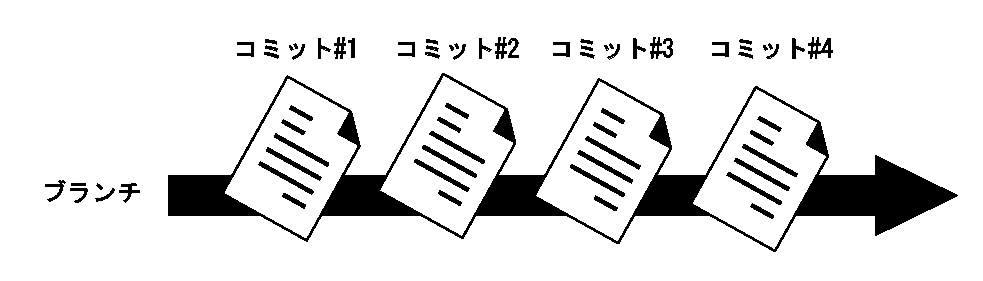
\includegraphics[width=75mm]{img/branch1.eps}
\caption{ブランチの概念}
\label{branch}
\end{figure}

ブランチとは,蓄積されたコミットの時系列と,系列を分岐する操作を指す.分岐したブランチ同士は互いに独立しており,任意のブランチ内のコミットは他のブランチでのコミットの影響を受けない.ブランチ同士の結合はマージと呼ぶ.

\subsubsection{バグ修正におけるブランチの有用性}
ブランチを利用した一例を以下の\fgref{branch_ex}に示す.

\begin{figure}[h]
\centering
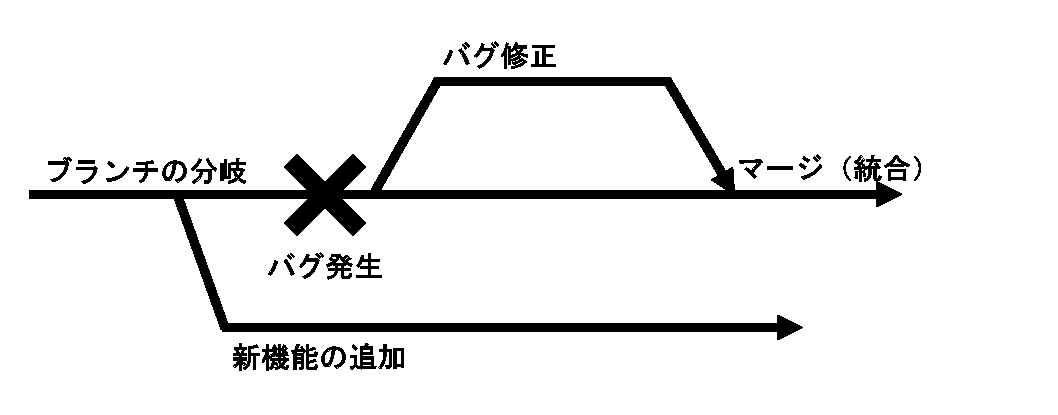
\includegraphics[width=80mm]{img/branch.eps}
\caption{ブランチの一例}
\label{branch_ex}
\end{figure}

ブランチを用いることで,様々な開発やバグ修正などを同時並行で行うことができる.具体的には,\fgref{branch_ex}において既に運用されているソフトウエアの管理を行っているブランチをmasterブランチとし,そのソフトウエアのバグを修正するために用意したブランチをbugfixブランチとする.この場合,二つのブランチは独立しているため,masterブランチに影響を与えることなくbugfixブランチでバグ修正を行うことができる.すなわち,ブランチを使用しない場合は,バグ修正が完了するまでソフトウエアの運用を停止しなければならないが,ブランチを用いることでソフトウエアの運用を止めることなく,平行してバグ修正を行うことができる.バグ修正が完了した後にマージを行えば,ソフトウエアの運用が行われたまま,マージの時点でバグが修正される.さらにブランチの本数を増やせば,リリースしたソフトウエアを運用しながら新機能の追加を行い,さらにバグ修正も同時並行で行うといった運用が可能である.

\subsection{内部処理}
内部処理・・・

\subsection{利点と欠点}
gitの利点は次の通りである.

\begin{itemize}
\item ローカルリポジトリを持つ
\item ブランチ機能が強力
\item 高速である
\end{itemize}

ローカルリポジトリによって,ネットワークに接続されていない環境でもコミットを行うことができる.あるいは,バグ修正のために個人のローカルリポジトリに適量のコミットを行い,修正が完了した後にリモートリポジトリにプッシュし他者に公開するといった使用方法が可能である.

さらに,ブランチ機能が他の他のバージョン管理システムに比べて優れている.他のシステムでは,マージの際にどのファイルをどのようにマージするか明示的に入力する必要があるが,gitは自動的に行う.また,マージにかかる時間も他のシステムに比べて高速である.

加えて,gitはC言語で記述されているため,全体の動作が他のシステムに比べて高速である.これは,gitがLinuxカーネル開発に使用するために開発されたため,OSカーネルのような巨大なソースコードの集合を高速に処理する必要があった経緯がある.

欠点は,gitで扱えるファイルの種類がテキストベースのファイルに限られる点である.このため,書類作成のデファクト・スタンダードである,Microsoft Officeで作成したファイルを改変なしでは管理できない.

\section{今後の展望}
今日,ソフトウエアのリリース速度は増加の一途をたどり,その裏では開発の効率化,高速化が重要視されている.そのため,gitのようなバージョン管理ソフトウエアやチケット駆動開発は更に普及すると考えられる.また,現在はGitHubのようなSNSサービスは概ね無料で公開されているが,あるソフトウエアの開発において,デバッグや開発の一部を他者に依頼し,一番良いソースコードを含むフォークに報酬を払うなどのビジネスも近い将来に生まれると考える.

\small
\begin{thebibliography}{99}

\end{thebibliography}


%
%\subsection{LEDの構造と発光原理}
%\fgref{led}を参照します.
%
%\begin{figure}[h]
%\centering
%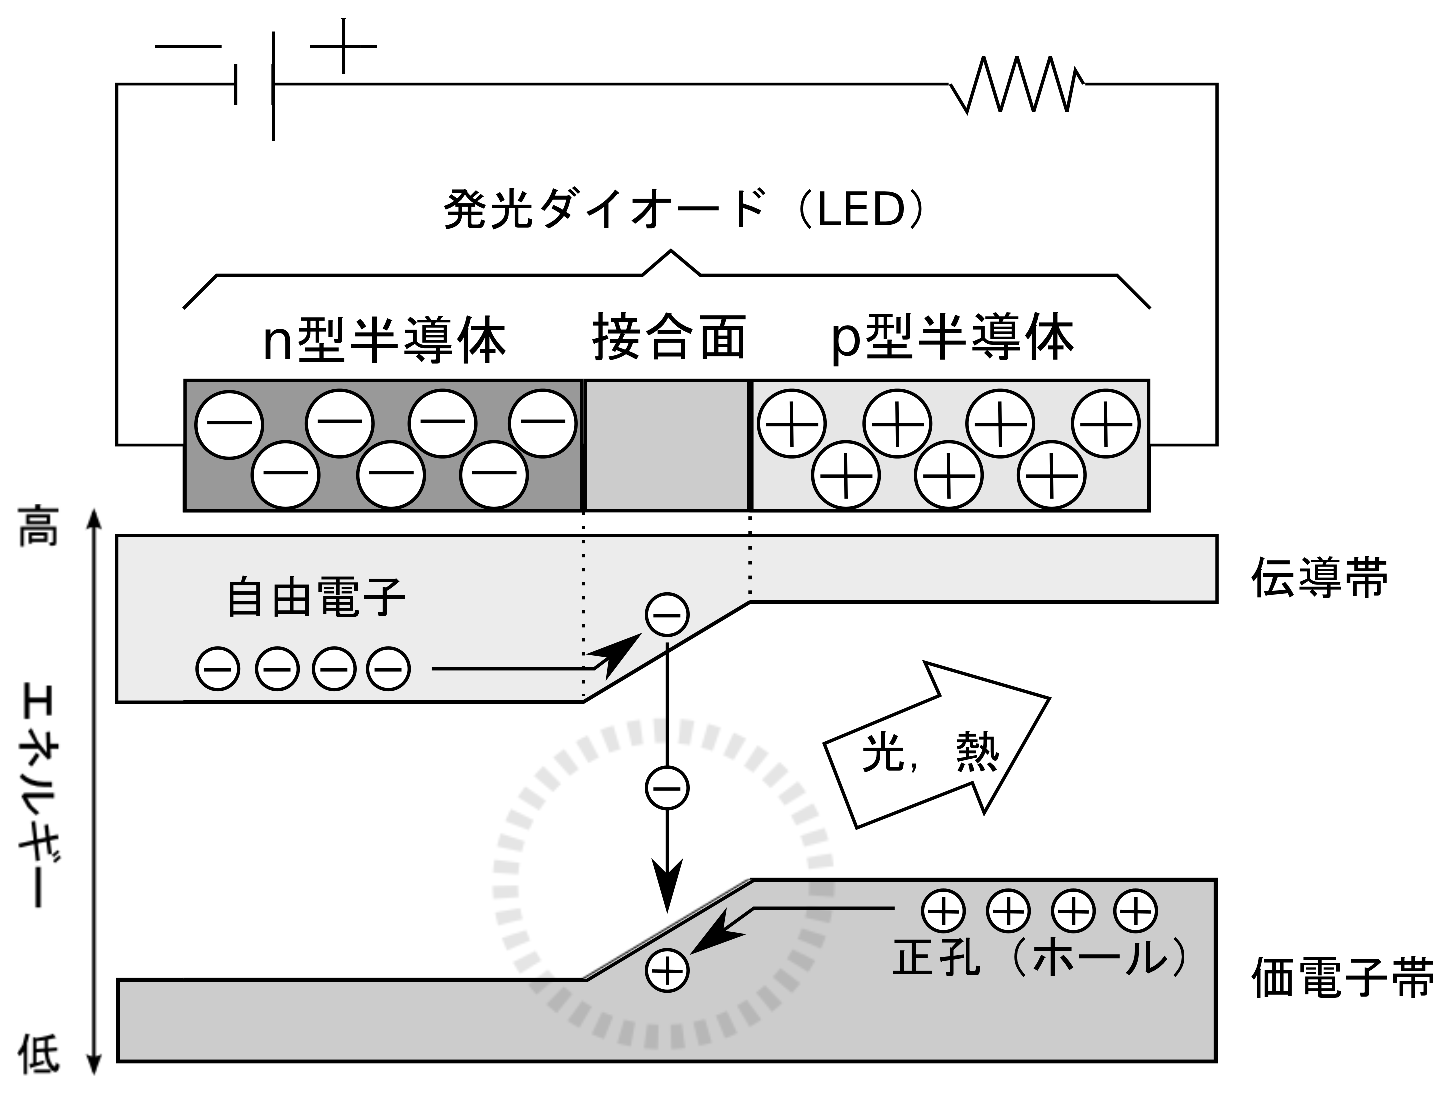
\includegraphics[width=80mm]{img/function.eps}
%\caption{参考画像1}
%\label{led}
%\end{figure}
%
%
%\fgref{sh}を参照します.
%
%\begin{figure}[h]
%
%\centering
%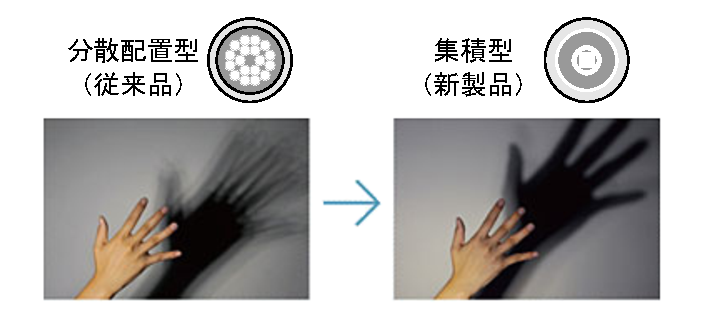
\includegraphics[width=80mm]{img/shade.eps}
%
%縦の空白を挿入する
%\vspace{3cm}
%
%
%\caption{参考画像2}
%\label{sh}
%\end{figure}
%
%
%\section{表を作る}
%
%\begin{table}[h]
%\caption{照明器具の性能比較(参考文献\cite{eru}を参照)}
%\label{table}
%\begin{tabular}{|c|l|l|l|}
%\hline
%  & 白熱電球 & 蛍光灯 & LED照明 \\ \hline
%寿命 & 1000時間 & 10000時間 & 40000時間 \\ \hline
%指向性 & なし & なし & あり\\ \hline
%発光効率 & 10 lm/W & 70 lm/W & 85 lm/W \\
% & & 〜100 lm/W & \\ \hline
%消費電力 & 54 W & 12 W & 7 W\\ \hline
%演色性 & 100 & 84 & 70〜90\\ 
%(Ra) & & & \\ \hline
%発光波長 & 赤外線が & 紫外線が & ほぼ\\
% & 多い & 多い & 可視光線のみ \\ \hline
%電源 & 交流 & 交流 & 直流 \\ \hline
%価格 & - & 白熱電球の & 白熱電球の \\
% & & 20倍 & 80倍 \\ \hline
%\end{tabular}
%\end{table}
%
%縦の空白を挿入する
%
%\tbref{table}を参照します.
%
%
%\vspace{3cm}
%
%\section{箇条書き}
%
%\begin{itemize}
%\item ユニキャスト:他にも
%\item マルチキャスト:「*」などの
%\item エニーキャスト:itemもあります
%\end{itemize}
%
%
%\begin{enumerate}
%\item ユニキャスト:このような
%\item マルチキャスト:番号付き箇条書きも
%\item エニーキャスト:可能です
%\end{enumerate}
%
%\small
%\begin{thebibliography}{99}
%
%\bibitem{SNtech}
%安藤繁,田村陽介,戸辺義人ほか:
%センサネットワーク技術-ユビキタス情報環境の構築に向けて,
%東京電機大学出版局(2005).
%
%\bibitem{reprogramming}
%Wang, Q. and Zhu, Y. and Cheng, L.:
%Reprogramming wireless sensor networks: challenges and approaches,
%{\it Network, IEEE},
%Vol.20,
%No.3,
%pp.48-55(2006).

%% -------------------

%\end{thebibliography}

%% \bibliographystyle{junsrt}
%% \bibliography{bibsample}
\end{document}
